% -*- mode: latex; -*- mustache tags:  
\documentclass[10pt,twoside,english]{_support/latex/sbabook/sbabook}
\let\wholebook=\relax

\usepackage{import}
\subimport{_support/latex/}{common.tex}

%=================================================================
% Debug packages for page layout and overfull lines
% Remove the showtrims document option before printing
\ifshowtrims
  \usepackage{showframe}
  \usepackage[color=magenta,width=5mm]{_support/latex/overcolored}
\fi


% =================================================================
\title{The Pharo object model}
\author{Stéphane Ducasse, Dimitris Chloupis, Nicolai Hess, and Dmitri Zagidulin\ (based on A.P. Black, S. Ducasse, O. Nierstrasz, D. Pollet, with D. Cassou and M. Denker)}
\series{The Pharo Technology Collection}

\hypersetup{
  pdftitle = {The Pharo object model},
  pdfauthor = {Stéphane Ducasse, Dimitris Chloupis, Nicolai Hess, and Dmitri Zagidulin\ (based on A.P. Black, S. Ducasse, O. Nierstrasz, D. Pollet, with D. Cassou and M. Denker)},
  pdfkeywords = {Pharo}
}


% =================================================================
\begin{document}

% Title page and colophon on verso
\maketitle
\pagestyle{titlingpage}
\thispagestyle{titlingpage} % \pagestyle does not work on the first one…

\cleartoverso
{\small

  Copyright 2017 by Stéphane Ducasse, Dimitris Chloupis, Nicolai Hess, and Dmitri Zagidulin\ (based on A.P. Black, S. Ducasse, O. Nierstrasz, D. Pollet, with D. Cassou and M. Denker).

  The contents of this book are protected under the Creative Commons
  Attribution-ShareAlike 3.0 Unported license.

  You are \textbf{free}:
  \begin{itemize}
  \item to \textbf{Share}: to copy, distribute and transmit the work,
  \item to \textbf{Remix}: to adapt the work,
  \end{itemize}

  Under the following conditions:
  \begin{description}
  \item[Attribution.] You must attribute the work in the manner specified by the
    author or licensor (but not in any way that suggests that they endorse you
    or your use of the work).
  \item[Share Alike.] If you alter, transform, or build upon this work, you may
    distribute the resulting work only under the same, similar or a compatible
    license.
  \end{description}

  For any reuse or distribution, you must make clear to others the
  license terms of this work. The best way to do this is with a link to
  this web page: \\
  \url{http://creativecommons.org/licenses/by-sa/3.0/}

  Any of the above conditions can be waived if you get permission from
  the copyright holder. Nothing in this license impairs or restricts the
  author's moral rights.

  \begin{center}
    
\includegraphics[width=0.2\textwidth]{_support/latex/sbabook/CreativeCommons-BY-SA.pdf}
  \end{center}

  Your fair dealing and other rights are in no way affected by the
  above. This is a human-readable summary of the Legal Code (the full
  license): \\
  \url{http://creativecommons.org/licenses/by-sa/3.0/legalcode}

  \vfill

  % Publication info would go here (publisher, ISBN, cover design…)
  Layout and typography based on the \textcode{sbabook} \LaTeX{} class by Damien
  Pollet.
}


\frontmatter
\pagestyle{plain}

\tableofcontents*
\clearpage\listoffigures

\mainmatter

\label{cha:model}
The Pharo programming model is heavily inspired by the one of Smalltalk. It is
simple and uniform: everything is an object, and objects communicate only by
sending each other messages. Instance variables are private to the object.
Methods are all public and dynamically looked up (late-bound). In this chapter
we present the core concepts of the Pharo object model. We revisit concepts such
as \textcode{self} and \textcode{super} and define precisely their semantics. Then we discuss
the consequences of representing classes as objects. This will be extended in
Chapter:
\hyperref[cha:metaclasses]{Classes and Metaclasses}.
\chapter{The rules of the model}\label{sec:rules}
The object model is based on a set of simple rules that are applied
\textit{uniformly}. The rules are as follows:

\textbf{Rule 1}. Everything is an object.

\textbf{Rule 2}. Every object is an instance of a class.

\textbf{Rule 3}. Every class has a superclass.

\textbf{Rule 4}. Everything happens by sending messages.

\textbf{Rule 5}. Method lookup dynamically follows the inheritance chain.

Let us look at each of these rules in some detail.
\chapter{Everything is an Object}
The mantra \textit{everything is an object} is highly contagious. After only a short
while working with Pharo, you will start to be surprised at how this rule
simplifes everything you do. Integers, for example, are truly objects, so you
can send messages to them, just as you do to any other object. At the end of
this chapter, we added an implementation note on the object implementation for
the curious reader.

\begin{displaycode}{plain}
"send '+ 4' to 3, yielding 7"
3 + 4
>>> 7
\end{displaycode}

\begin{displaycode}{plain}
"send factorial, yielding a big number"
20 factorial
>>> 2432902008176640000
\end{displaycode}

The object \textcode{7} is different than the object returned by \textcode{20 factorial}, but
because they are both polymorphic objects, none of the code, not even the
implementation of \textcode{factorial}, needs to know about this.

Coming back to \textit{everything is an object} rule, perhaps the most fundamental
consequence of this rule is that classes are objects too. Classes are not
second-class objects: they are really first-class objects that you can send
messages to, inspect, and change. This means that Pharo is a truly reflective
system, which gives a great deal of expressive power to developers.

\begin{important}
Classes are objects too.
\end{important}
\chapter{Every object is an instance of a class}
Every object has a class; you can find out which one by sending it the message
\textcode{class}.

\begin{displaycode}{plain}
1 class
>>> SmallInteger
\end{displaycode}

\begin{displaycode}{plain}
20 factorial class
>>> LargePositiveInteger
\end{displaycode}

\begin{displaycode}{plain}
'hello' class
>>> ByteString
\end{displaycode}

\begin{displaycode}{plain}
(4@5) class
>>> Point
\end{displaycode}

\begin{displaycode}{plain}
Object new class
>>> Object
\end{displaycode}

A class defines the \textit{structure} of its instances via instance variables, and
the \textit{behavior} of its instances via methods. Each method has a name, called
its \textit{selector}, which is unique within the class.

Since \textit{classes are objects}, and \textit{every object is an instance of a class},
it follows that classes must also be instances of classes. A class whose
instances are classes is called a \textit{metaclass}. Whenever you create a class,
the system automatically creates a metaclass for you. The metaclass defines the
structure and behavior of the class that is its instance. 99\% of the time you
will not need to think about metaclasses, and may happily ignore them. (We will
have a closer look at metaclasses in Chapter
\hyperref[cha:metaclasses]{: Classes and Metaclasses}.)
\chapter{Instance structure and behavior}
Now we will briefly present how we specify the structure and behavior of
instances.
\section{Instance variables}
Instance variables in Pharo are private to the \textit{instance} itself. This is in
contrast to Java and C++, which allow instance variables (also known as
\textit{fields} or \textit{member variables}) to be accessed by any other instance that
happens to be of the same class. We say that the \textit{encapsulation boundary} of
objects in Java and C++ is the class, whereas in Pharo it is the instance.

In Pharo, two instances of the same class cannot access each other's instance
variables unless the class defines \textit{accessor methods}. There is no language
syntax that provides direct access to the instance variables of any other
object. (Actually, a mechanism called reflection does provide a way to ask
another object for the values of its instance variables; meta-programming is
intended for writing tools like the object inspector, whose sole purpose is to
look inside other objects.)

Instance variables can be accessed by name in any of the instance methods of the
class that defines them, and also in the methods defined in its subclasses. This
means that Pharo instance variables are similar to \textit{protected} variables in
C++ and Java. However, we prefer to say that they are private, because it is
considered bad style in Pharo to access an instance variable directly from a
subclass.
\subsection{Instance encapsulation example}
The method \textcode{Point\textgreater{}\textgreater{}dist:} computes the distance between the receiver and
another point. The instance variables \textcode{x} and \textcode{y} of the receiver are
accessed directly by the method body. However, the instance variables of the
other point must be accessed by sending it the messages \textcode{x} and \textcode{y}.

\begin{listing}[float, label=scr:distance]{plain}{Distance between two points}
Point >> dist: aPoint
    "Answer the distance between aPoint and the receiver."

    | dx dy |
    dx := aPoint x - x.
    dy :=  aPoint y - y.
    ^ ((dx * dx) + (dy * dy)) sqrt
\end{listing}

\begin{displaycode}{plain}
1@1 dist: 4@5
>>> 5.0
\end{displaycode}

The key reason to prefer instance-based encapsulation to class-based
encapsulation is that it enables different implementations of the same
abstraction to coexist. For example, the method \textcode{dist:} need not know or care
whether the argument \textcode{aPoint} is an instance of the same class as the
receiver. The argument object might be represented in polar coordinates, or as a
record in a database, or on another computer in a distributed system. As long as
it can respond to the messages \textcode{x} and \textcode{y}, the code of method \textcode{dist}
(shown above) will still work.
\section{Methods}
All methods are \textit{public} and virtual (i.e., dynamically looked up). Methods
are grouped into \textit{protocols} that indicate their intent. Some common protocol
names have been established by convention, for example, \textcode{accessing} for all
accessor methods, and \textcode{initialization} for establishing a consistent initial
state for the object. The protocol \textcode{private} is sometimes used to group
methods that should not be seen from outside. Nothing, however, prevents you
from sending a message that is implemented by such a \symbol{34}private\symbol{34} method.

Methods can access all instance variables of the object. Some developers prefer
to access instance variables only through accessors. This practice has some
value, but it also clutters the interface of your classes, and worse, exposes
its private state to the world.
\chapter{The instance side and the class side}
Since classes are objects, they can have their own instance variables and their
own methods. We call these \textit{class instance variables} and \textit{class methods},
but they are really no different from ordinary instance variables and methods:
They simply operate on different objects (classes in this case). An instance
variable describes instance state and a method describes instance behavior.
Similarly, class instance variables are just instance variables defined by a
metaclass (and describe the state of classes - instances of metaclasses), and
class methods are just methods defined by a metaclass (and that will be executed
on classes).

A class and its metaclass are two separate classes, even though the former is an
instance of the latter. However, this is largely irrelevant to you as a
programmer: you are concerned with defining the behavior of your objects and the
classes that create them.


\begin{figure}

\begin{center}
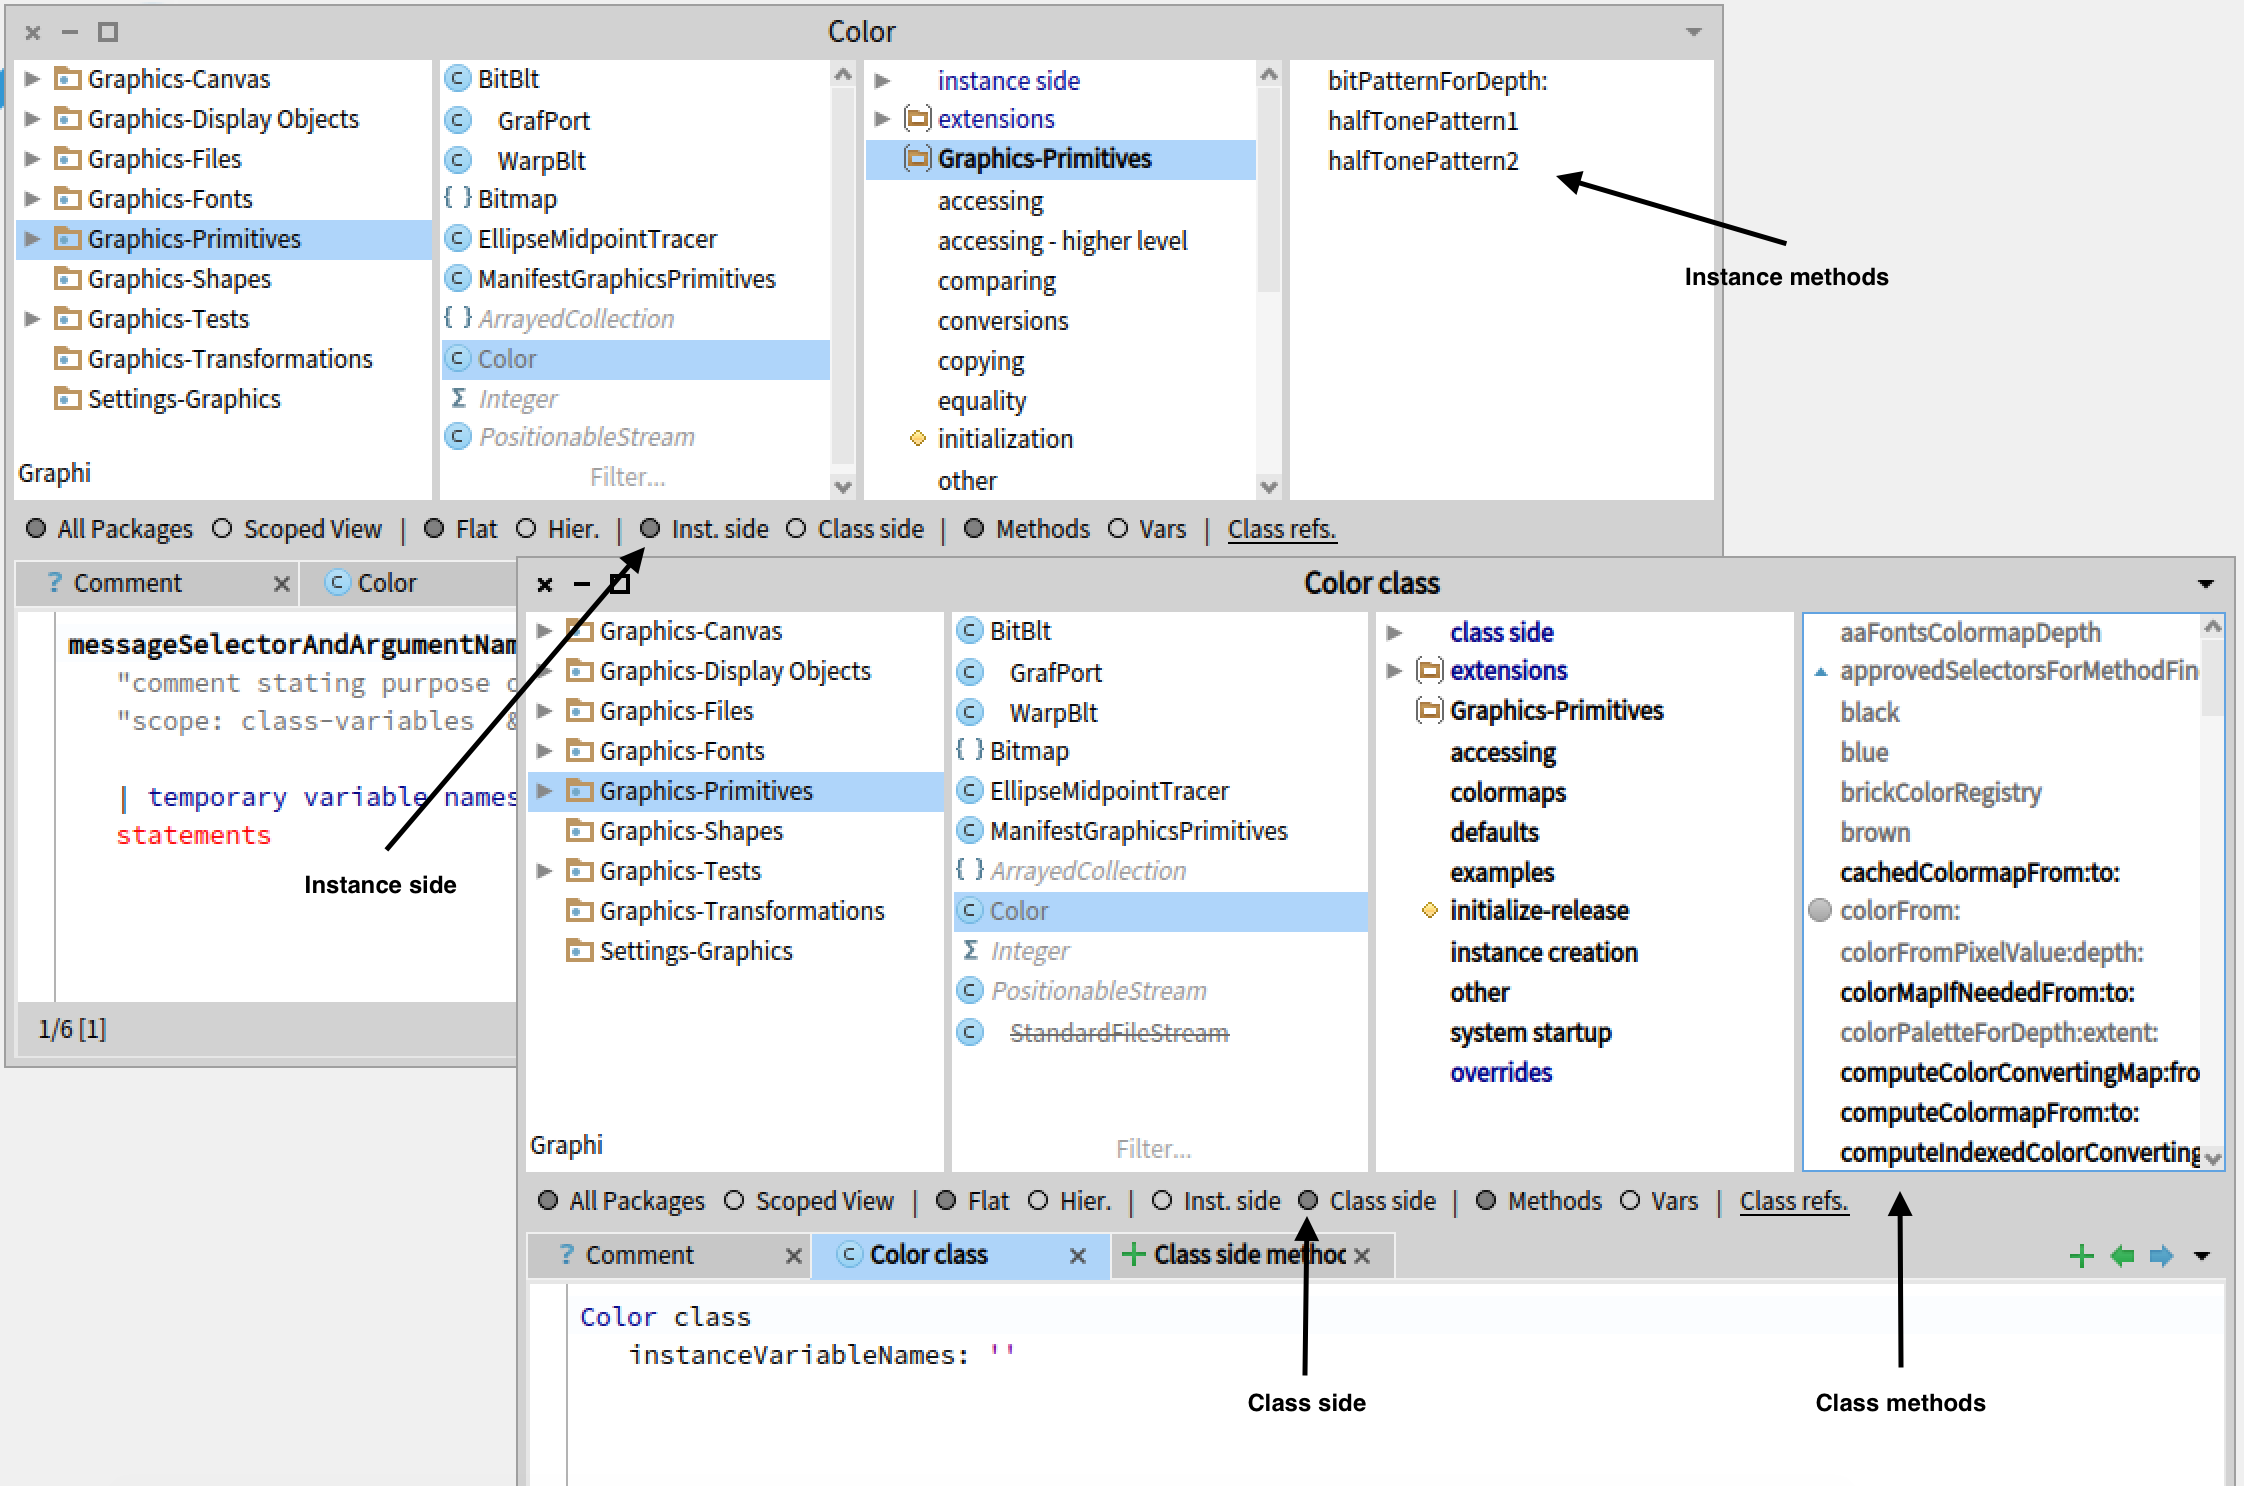
\includegraphics[width=0.9\textwidth]{/Users/sebastijan.kaplar/Desktop/PharoByExample/UpdatedPharoByExample/_result/pdf/PharoObjectModel/figures/colorInstanceClassSide.png}\caption{Browsing a class and its metaclass\label{fig:colorInstanceClassSide}}\end{center}
\end{figure}


For this reason, the browser helps you to browse both class and metaclass as if
they were a single thing with two \symbol{34}sides\symbol{34}: the \textit{instance side} and the \textit{class
side}, as shown in Figure \ref{fig:colorInstanceClassSide}. By default, when you
select a class in the browser, you're browsing the \textit{instance} side (i.e., the
methods that are executed when messages are sent to an \textit{instance} of
\textcode{Color}). Clicking on the \textbf{Class side} button switches you over to the
\textit{class side} (the methods that will be executed when messages are sent to the
\textit{class} \textcode{Color} itself).

For example, \textcode{Color blue} sends the message \textcode{blue} to the class \textcode{Color}.
You will therefore find the method \textcode{blue} defined on the class side of
\textcode{Color}, not on the instance side.

\begin{displaycode}{plain}
"Class-side method blue (convenient instance creation method)"
aColor := Color blue.
>>> Color blue
"Color instances are self-evaluating"
\end{displaycode}

\begin{displaycode}{plain}
"Instance-side accessor method red (returns the red RGB value)"
Color blue red
>>> 0.0
\end{displaycode}

\begin{displaycode}{plain}
"Instance-side accessor method blue (returns the blue RGB value)"
Color blue blue
>>> 1.0
\end{displaycode}

You define a class by filling in the template proposed on the instance side.
When you accept this template, the system creates not just the class that you
defined, but also the corresponding metaclass (which you can then edit by
clicking on the \textbf{Class side} button). The only part of the metaclass creation
template that makes sense for you to edit directly is the list of the
metaclass's instance variable names.

Once a class has been created, browsing its instance side (\textbf{Class side}
un-checked) lets you edit and browse the methods that will be possessed by
instances of that class (and of its subclasses).
\section{Class methods}
Class methods can be quite useful; browse \textcode{Color class} for some good
examples. You will see that there are two kinds of methods defined on a class:
\textit{instance creation methods}, like \textcode{Color class\textgreater{}\textgreater{}blue}, and those that
perform a utility function, like \textcode{Color class\textgreater{}\textgreater{}wheel:}. This is typical,
although you will occasionally find class methods used in other ways.

It is convenient to place utility methods on the class side because they can be
executed without having to create any additional objects first. Indeed, many of
them will contain a comment designed to make it easy to execute them.

Browse method \textcode{Color class\textgreater{}\textgreater{}wheel:}, double-click just at the beginning of the
comment \textcode{\symbol{34}(Color wheel: 12) inspect\symbol{34}} and press \textcode{CMD-d}. You will see the
effect of executing this method.

For those familiar with Java and C++, class methods may seem similar to static
methods. However, the uniformity of the Pharo object model (where classes are
just regular objects) means that they are somewhat different: whereas Java
static methods are really just statically-resolved procedures, Pharo class
methods are dynamically-dispatched methods. This means that inheritance,
overriding and super-sends work for class methods in Pharo, whereas they don't
work for static methods in Java.
\section{Class instance variables}
With ordinary instance variables, all the instances of a class have the same set
of variable names (though each instance has its own private set of values), and
the instances of its subclasses inherit those names. The story is exactly the
same with class instance variables: each class has its own private class
instance variables. A subclass will inherit those class instance variables,
\textit{but the subclass will have its own private copies of those variables}. Just
as objects don't share instance variables, neither do classes and their
subclasses share class instance variables.

For example, you could use a class instance variable called \textcode{count} to keep
track of how many instances you create of a given class. However, any subclass
would have its own \textcode{count} variable, so subclass instances would be counted
separately.
\subsection{Example: Class instance variables and subclasses}
Suppose we define the class \textcode{Dog}, and its subclass \textcode{Hyena}. Suppose that we
add a \textcode{count} class instance variable to the class \textcode{Dog} (i.e. we define it
on the metaclass \textcode{Dog class}). \textcode{Hyena} will naturally inherit the class
instance variable \textcode{count} from \textcode{Dog}.

\begin{listing}[float]{plain}{Dogs and Hyenas}
Object subclass: #Dog
    instanceVariableNames: ''
    classVariableNames: ''
    package: 'PBE-CIV'
\end{listing}

\begin{displaycode}{plain}
Dog class
    instanceVariableNames: 'count'
\end{displaycode}

\begin{displaycode}{plain}
Dog subclass: #Hyena
    instanceVariableNames: ''
    classVariableNames: ''
    package: 'PBE-CIV'
\end{displaycode}

Now suppose we define class methods for \textcode{Dog} to initialize its \textcode{count} to
\textcode{0}, and to increment it when new instances are created:

\begin{listing}[float, label=scr:dogCount]{plain}{Keeping count of new dogs}
Dog class >> initialize
    count := 0.
\end{listing}

\begin{displaycode}{plain}
Dog class >> new
    count := count +1.
    ^ super new
\end{displaycode}

\begin{displaycode}{plain}
Dog class >> count
    ^ count
\end{displaycode}

Now when we create a new \textcode{Dog}, the \textcode{count} value of the class \textcode{Dog} is
incremented, and so is that of the class \textcode{Hyena} (but the hyenas are counted
separately).

\textit{Side note:} Notice the use of \textcode{initialize} on the classes, in the following
code. In Pharo, when you instantiate an object such as \textcode{Dog new},
\textcode{initialize} is called automatically as part of the \textcode{new} message send (you
can see for yourself by browsing \textcode{Behavior\textgreater{}\textgreater{}new}). But with classes, simply
defining them does not automatically call \textcode{initialize}, and so we have to call
it explicitly here. By default class initialize methods are automatically
executed only when classes are loaded. See also the discussion about lazy
initialization, below.

\begin{listing}[float, label=scr:dogCount2]{plain}{}
Dog initialize.
Hyena initialize.
Dog count
>>> 0
\end{listing}

\begin{displaycode}{plain}
Hyena count
>>> 0
\end{displaycode}

\begin{displaycode}{plain}
| aDog |
aDog := Dog new.
Dog count
>>> 1  "Incremented"
\end{displaycode}

\begin{displaycode}{plain}
Hyena count
>>> 0  "Still the same"
\end{displaycode}

Class instance variables are private to a class in exactly the same way that
instance variables are private to an instance. Since classes and their
instances are different objects, this has the following consequences:

\textbf{1.} A class does not have access to the instance variables of its own
instances. So, the class \textcode{Color} does not have access to the variables of an
object instantiated from it, \textcode{aColorRed}. In other words, just because a class
was used to create an instance (using \textcode{new} or a helper instance creation
method like \textcode{Color red}), it doesn't give \textit{the class} any special direct
access to that instance's variables. The class instead has to go through the
accessor methods (a public interface) just like any other object.

\textbf{2.} The reverse is also true: an \textit{instance} of a class does not have access
to the class instance variables of its class. In our example above, \textcode{aDog}
(an individual instance) does not have direct access to the \textcode{count} variable
of the \textcode{Dog} class (except, again, through an accessor method).

\begin{important}
A class does not have access to the instance variables of its own instances. An instance of a class does not have access to the class instance variables of its class.
\end{important}

For this reason, instance initialization methods must always be defined on the
instance side, the class side has no access to instance variables, and so cannot
initialize them! All that the class can do is to send initialization messages,
using accessors, to newly created instances.

Java has nothing equivalent to class instance variables. Java and C++ static
variables are more like Pharo class variables (discussed in
Section \ref{sec:classVars}), since in those languages all of the subclasses and
all of their instances share the same static variable.
\subsection{Example: Defining a Singleton}
The Singleton pattern provides a typical example of the use of class instance
variables and class methods. Imagine that we would like to implement a class
\textcode{WebServer}, and to use the Singleton pattern to ensure that it has only one
instance.

We define the class \textcode{WebServer} as follow.

\begin{listing}[float]{plain}{A sample singleton class, \textcode{WebServer}}
Object subclass: #WebServer
    instanceVariableNames: 'sessions'
    classVariableNames: ''
    package: 'Web'
\end{listing}

Then, clicking on the \textbf{Class side} button, we add the (class) instance
variable \textcode{uniqueInstance}.

\begin{listing}[float]{plain}{The class side of the singleton class}
WebServer class
    instanceVariableNames: 'uniqueInstance'
\end{listing}

As a result, the class \textcode{WebServer class} will have a new instance variable (in
addition to the variables that it inherits from \textcode{Behavior}, such as
\textcode{superclass} and \textcode{methodDict}). It means that the value of this extra
instance variable will describe the instance of the class \textcode{WebServer class}
i.e. the class \textcode{WebServer}.

\begin{listing}[float, label=scr:instance]{plain}{New state for classes}
Object class allInstVarNames
>>>  "#('superclass' 'methodDict' 'format' 'layout' 'instanceVariables' 'organization' 'subclasses' 'name' 'classPool' 'sharedPools' 'environment' 'category' 'traitComposition' 'localSelectors')"
\end{listing}

\begin{displaycode}{plain}
WebServer class allInstVarNames
>>>"#('superclass' 'methodDict' 'format' 'layout' 'instanceVariables' 'organization' 'subclasses' 'name' 'classPool' 'sharedPools' 'environment' 'category' 'traitComposition' 'localSelectors' #uniqueInstance)"
\end{displaycode}

We can now define a class method named \textcode{uniqueInstance}, as shown below. This
method first checks whether \textcode{uniqueInstance} has been initialized. If it has
not, the method creates an instance and assigns it to the class instance
variable \textcode{uniqueInstance}. Finally the value of \textcode{uniqueInstance} is
returned. Since \textcode{uniqueInstance} is a class instance variable, this method can
directly access it.

\begin{listing}[float, label=scr:uniqueInstance]{smalltalk}{Class-side accessor method \textcode{uniqueInstance}}
WebServer class >> uniqueInstance
     uniqueInstance ifNil: [ uniqueInstance := self new ].
     ^ uniqueInstance
\end{listing}

The first time that \textcode{WebServer uniqueInstance} is executed, an instance of the
class \textcode{WebServer} will be created and assigned to the \textcode{uniqueInstance}
variable. The next time, the previously created instance will be returned
instead of creating a new one. (This pattern, checking if a variable is nil
in an accessor method, and initializing its value if it is nil, is called
\textit{lazy initialization}).

Note that the instance creation code in the code above.

is written as \textcode{self new} and not as \textcode{WebServer new}. What is the difference?
Since the \textcode{uniqueInstance} method is defined in \textcode{WebServer class}, you might
think that there is no difference. And indeed, until someone creates a subclass
of \textcode{WebServer}, they are the same. But suppose that \textcode{ReliableWebServer} is
a subclass of \textcode{WebServer}, and inherits the \textcode{uniqueInstance} method. We
would clearly expect \textcode{ReliableWebServer uniqueInstance} to answer a
\textcode{ReliableWebServer}. Using \textcode{self} ensures that this will happen, since
\textcode{self} will be bound to the respective receiver, here the classes
\textcode{WebServer} and \textcode{ReliableWebServer}. Note also that \textcode{WebServer} and
\textcode{ReliableWebServer} will each have a different value for their
\textcode{uniqueInstance} instance variable.
\subsubsection{A note on lazy initialization.}
\textit{Do not over-use the lazy initialization pattern.} The setting of initial
values for instances of objects generally belongs in the \textcode{initialize} method.
Putting initialization calls only in \textcode{initialize} helps from a readability
perspective -- you don't have to hunt through all the accessor methods to see
what the initial values are. Although it may be tempting to instead initialize
instance variables in their respective accessor methods (using \textcode{ifNil:}
checks), avoid this unless you have a good reason.

For example, in our \textcode{uniqueInstance} method above, we used lazy initialization
because users won't typically expect to call \textcode{WebServer initialize}. Instead,
they expect the class to be \symbol{34}ready\symbol{34} to return new unique instances. Because of
this, lazy initialization makes sense. Similarly, if a variable is expensive to
initialize (opening a database connection or a network socket, for example),
you will sometimes choose to delay that initialization until you actually need
it.
\chapter{Every class has a superclass}
Each class in Pharo inherits its behaviour and the description of its
structure from a single \textit{superclass}. This means that Smalltalk has single
inheritance.

\begin{displaycode}{plain}
SmallInteger superclass
>>> Integer
\end{displaycode}

\begin{displaycode}{plain}
Integer superclass
>>> Number
\end{displaycode}

\begin{displaycode}{plain}
Number superclass
>>> Magnitude
\end{displaycode}

\begin{displaycode}{plain}
Magnitude superclass
>>> Object
\end{displaycode}

\begin{displaycode}{plain}
Object superclass
>>> ProtoObject
\end{displaycode}

\begin{displaycode}{plain}
ProtoObject superclass
>>> nil
\end{displaycode}

Traditionally the root of an inheritance hierarchy is the class \textcode{Object}
(since everything is an object). In Pharo, the root is actually a class called
\textcode{ProtoObject}, but you will normally not pay any attention to this class.
\textcode{ProtoObject} encapsulates the minimal set of messages that all objects
\textit{must} have and \textcode{ProtoObject} is designed to raise as many as possible
errors (to support proxy definition). However, most classes inherit from
\textcode{Object}, which defines many additional messages that almost all objects
understand and respond to. Unless you have a very good reason to do otherwise,
when creating application classes you should normally subclass \textcode{Object}, or
one of its subclasses.

A new class is normally created by sending the message \textcode{subclass:
instanceVariableNames: ...} to an existing class. There are a few other methods
to create classes. To see what they are, have a look at \textcode{Class} and its
\textcode{subclass creation} protocol.

Although Pharo does not provide multiple inheritance, it supports a mechanism
called Traits for sharing behaviour across unrelated classes. Traits are
collections of methods that can be reused by multiple classes that are not
related by inheritance. Using traits allows one to share code between different
classes without duplicating code.
\section{Abstract methods and abstract classes}
An abstract class is a class that exists to be subclassed, rather than to be
instantiated. An abstract class is usually incomplete, in the sense that it does
not define all of the methods that it uses. The \symbol{34}placeholder\symbol{34} methods, those
that the other methods assume to be (re)defined are called abstract methods.

Pharo has no dedicated syntax to specify that a method or a class is abstract.
Instead, by convention, the body of an abstract method consists of the
expression \textcode{self subclassResponsibility}. This indicates that subclasses have
the responsibility to define a concrete version of the method. \textcode{self
subclassResponsibility} methods should always be overridden, and thus should
never be executed. If you forget to override one, and it is executed, an
exception will be raised.

Similarly, a class is considered abstract if one of its methods is abstract.
Nothing actually prevents you from creating an instance of an abstract class;
everything will work until an abstract method is invoked.
\subsection{Example: the abstract class \textcode{Magnitude}}
\textcode{Magnitude} is an abstract class that helps us to define objects that can be
compared to each other. Subclasses of \textcode{Magnitude} should implement the
methods \textcode{\textless{}}, \textcode{}= and \textcode{hash}. Using such messages, \textcode{Magnitude} defines
other methods such as \textcode{\textgreater{}}, \textcode{\textgreater{}}=, \textcode{\textless{}}=, \textcode{max:}, \textcode{min:}
\textcode{between:and:} and others for comparing objects. Such methods are inherited
by subclasses. The method \textcode{Magnitude\textgreater{}\textgreater{}\textless{}} is abstract, and defined as shown in
the following script.

\begin{listing}[float, label=scr:MagnitudeLessThan]{plain}{\textcode{Magnitude\textgreater{}\textgreater{} \textless{}}}
< aMagnitude
    "Answer whether the receiver is less than the argument."

    ^self subclassResponsibility
\end{listing}

By contrast, the method \textcode{\textgreater{}}= is concrete, and is defined in terms of \textcode{\textless{}}.

\begin{listing}[float, label=scr:MagnitudeGTE]{plain}{\textcode{Magnitude\textgreater{}\textgreater{} \textgreater{}}=}
>= aMagnitude
    "Answer whether the receiver is greater than or equal to the argument."

    ^(self < aMagnitude) not
\end{listing}

The same is true of the other comparison methods (they are all defined in terms
of the abstract method \textcode{\textless{}}).

\textcode{Character} is a subclass of \textcode{Magnitude}; it overrides the
\textcode{\textless{}} method (which, if you recall, is marked as abstract in \textcode{Magnitude} by
the use of \textcode{self subclassResponsibility}) with its own version (see the
method definition below).

\textcode{Character} also explicitly defines methods
\textcode{}= and \textcode{hash}; it inherits from \textcode{Magnitude} the methods \textcode{\textgreater{}}=, \textcode{\textless{}}=,
\textcode{\textasciitilde{}}= and others.

\begin{listing}[float, label=scr:characterLessThan]{plain}{\textcode{Character\textgreater{}\textgreater{} \textless{}}=}
< aCharacter
    "Answer true if the receiver's value < aCharacter's value."

    ^self asciiValue < aCharacter asciiValue
\end{listing}
\section{Traits}
A \textit{trait} is a collection of methods that can be included in the behaviour of
a class without the need for inheritance. This makes it easy for classes to have
a unique superclass, yet still share useful methods with otherwise unrelated
classes.

To define a new trait, simply right-click in the class pane and select
\textcode{Add Trait}, or replace the subclass creation template by the trait
creation template, below.

\begin{listing}[float, label=scr:tauthor]{plain}{Defining a new trait}
Trait named: #TAuthor
    uses: { }
    package: 'PBE-LightsOut'
\end{listing}

Here we define the trait \textcode{TAuthor} in the package \textcode{PBE-LightsOut}. This
trait does not \textit{use} any other existing traits. In general we can specify a
\textit{trait composition expression} of other traits to use as part of the \textcode{uses:}
keyword argument. Here we simply provide an empty array.

Traits may contain methods, but no instance variables. Suppose we would like to
be able to add an \textcode{author} method to various classes, independent of where
they occur in the hierarchy.

We might do this as follows:

\begin{listing}[float, label=scr:author]{plain}{An author method}
TAuthor >> author
    "Returns author initials"

    ^ 'on'    "oscar nierstrasz"
\end{listing}

Now we can use this trait in a class that already has its own superclass, for
instance the \textcode{LOGame} class that we defined in Chapter \hyperref[cha:firstApp]{: A First Application}. We
simply modify the class creation template for \textcode{LOGame} to include a \textcode{uses:}
keyword argument that specifies that \textcode{TAuthor} should be used.

\begin{listing}[float, label=scr:sbegamewithtrait]{plain}{Using a trait}
BorderedMorph subclass: #LOGame
    uses: TAuthor
    instanceVariableNames: 'cells'
    classVariableNames: ''
    package: 'PBE-LightsOut'
\end{listing}

If we now instantiate \textcode{LOGame}, it will respond to the \textcode{author} message as
expected.

\begin{displaycode}{plain}
LOGame new author
>>> 'on'
\end{displaycode}

Trait composition expressions may combine multiple traits using the \textcode{+}
operator. In case of conflicts (i.e., if multiple traits define methods with
the same name), these conflicts can be resolved by explicitly removing these
methods (with \textcode{-}), or by redefining these methods in the class or trait that
you are defining. It is also possible to \textit{alias} methods (with \textcode{@}),
providing a new name for them.

Traits are used in the system kernel. One good example is the class
\textcode{Behavior}.

\begin{listing}[float, label=scr:behaviorwithtraits]{plain}{Behavior defined using traits}
Object subclass: #Behavior
    uses: TPureBehavior @ {#basicAddTraitSelector:withMethod:->#addTraitSelector:withMethod:}
    instanceVariableNames: 'superclass methodDict format'
    classVariableNames: 'ObsoleteSubclasses'
    package: 'Kernel-Classes'
\end{listing}

Here we see that the method \textcode{addTraitSelector:withMethod:} defined in the
trait \textcode{TPureBehavior} has been aliased to
\textcode{basicAddTraitSelector:withMethod:}.
\chapter{Everything happens by sending messages}
This rule captures the essence of programming in Pharo.

In procedural programming (and in some static features of some object-oriented
languages such as Java), the choice of which piece of code to execute when a
procedure is called is made by the caller. The caller chooses the procedure to
execute \textit{statically}, by name.

In Pharo, we do \textit{not} \symbol{34}invoke methods\symbol{34}. Instead, we \textit{send messages.} This is
just a terminology point but it is significant. It implies that this is not the
responsibility of the client to select the method to be executed, it is the one
of the receiver of the message.

When sending a message, we do not decide which method will be executed. Instead,
we \textit{tell} an object to do something for us by sending it a message. A message
is nothing but a name and a list of arguments. The receiver then decides how to
respond by selecting its own \textit{method} for doing what was asked. Since
different objects may have different methods for responding to the same message,
the method must be chosen \textit{dynamically}, when the message is received.

\begin{displaycode}{plain}
3 + 4
>>> 7          "send message + with argument 4 to integer 3"
\end{displaycode}

\begin{displaycode}{plain}
(1@2) + 4
>>> 5@6    "send message + with argument 4 to point (1@2)"
\end{displaycode}

As a consequence, we can send the \textit{same message} to different objects, each of
which may have \textit{its own method} for responding to the message. We do not tell
the \textcode{SmallInteger} \textcode{3} or the \textcode{Point} \textcode{(1@2)} how to respond to the
message \textcode{+ 4}. Each has its own method for \textcode{+}, and responds to \textcode{+ 4}
accordingly.

One of the consequences of Pharo's model of message sending is that it
encourages a style in which objects tend to have very small methods and delegate
tasks to other objects, rather than implementing huge, procedural methods that
assume too much responsibility. Joseph Pelrine expresses this principle
succinctly as follows:

\textit{\symbol{34}Don't do anything that you can push off onto someone else.\symbol{34}}

Many object-oriented languages provide both static and dynamic operations for
objects. In Pharo there are only dynamic message sends. For example, instead of
providing static class operations, we simply send messages to classes (which
are simply objects).

Ok, so \textit{nearly} everything in Pharo happens by sending messages. At some point
action must take place:

\textit{Variable declarations} are not message sends. In fact, variable declarations
are not even executable. Declaring a variable just causes space to be allocated
for an object reference.

\textit{Assignments} are not message sends. An assignment to a variable causes that
variable name to be freshly bound in the scope of its definition.

\textit{Returns} are not message sends. A return simply causes the computed result to
be returned to the sender.

\textit{Primitives} (and Pragmas/annotations) are not message sends. They are
implemented in the virtual machine.

Other than these few exceptions, pretty much everything else does truly happen
by sending messages. In particular, since there are no \textit{public fields} in
Pharo, the only way to update an instance variable of another object is to send
it a message asking that it update its own field. Of course, providing setter
and getter methods for all the instance variables of an object is not good
object-oriented style. Joseph Pelrine also states this very nicely:

\textit{\symbol{34}Don't let anyone else play with your data.\symbol{34}}
\chapter{Method lookup follows the inheritance chain}
What exactly happens when an object receives a message?
This is a two step process: method lookup and method execution.

\textbf{Lookup.} First, the method having the same name as the message is looked up.

\textbf{Method Execution.} Second, the found method is applied to the receiver with
the message arguments: When the method is found, the arguments are bound to the
parameters of the method, and the virtual machine executes it.

The lookup process is quite simple:

\textbf{1.} The class of the receiver looks up the method to use to handle the
message.

\textbf{2.} If this class does not have that method method defined, it asks its
superclass, and so on, up the inheritance chain.

It is essentially as simple as that. Nevertheless there are a few questions that
need some care to answer:

\begin{itemize}
\item \textit{What happens when a method does not explicitly return a value?}
\item \textit{What happens when a class reimplements a superclass method?}
\item \textit{What is the difference between \textcode{self} and \textcode{super} sends?}
\item \textit{What happens when no method is found?}
\end{itemize}

The rules for method lookup that we present here are conceptual; virtual machine
implementors use all kinds of tricks and optimizations to speed up method
lookup. That's their job, but you should never be able to detect that they are
doing something different from our rules.

First let us look at the basic lookup strategy, and then consider these further
questions.
\section{Method lookup}
Suppose we create an instance of \textcode{EllipseMorph}.

\begin{displaycode}{plain}
anEllipse := EllipseMorph new.
\end{displaycode}

If we now send this object the message \textcode{defaultColor}, we get the result
\textcode{Color yellow}.

\begin{displaycode}{plain}
anEllipse defaultColor
>>> Color yellow
\end{displaycode}

The class \textcode{EllipseMorph} implements \textcode{defaultColor}, so the appropriate
method is found immediately.

\begin{listing}[float, label=scr:defaultColor]{plain}{A locally implemented method}
EllipseMorph >> defaultColor
     "Answer the default color/fill style for the receiver"
     ^ Color yellow
\end{listing}

In contrast, if we send the message \textcode{openInWorld} to \textcode{anEllipse}, the method
is not immediately found, since the class \textcode{EllipseMorph} does not implement
\textcode{openInWorld}. The search therefore continues in the superclass,
\textcode{BorderedMorph}, and so on, until an \textcode{openInWorld} method is found in the
class \textcode{Morph} (see Figure \ref{fig:openInWorldLookup}).

\begin{listing}[float, label=scr:openInWorld]{plain}{An inherited method}
Morph >> openInWorld
     "Add this morph to the world."
     self openInWorld: self currentWorld
\end{listing}


\begin{figure}

\begin{center}
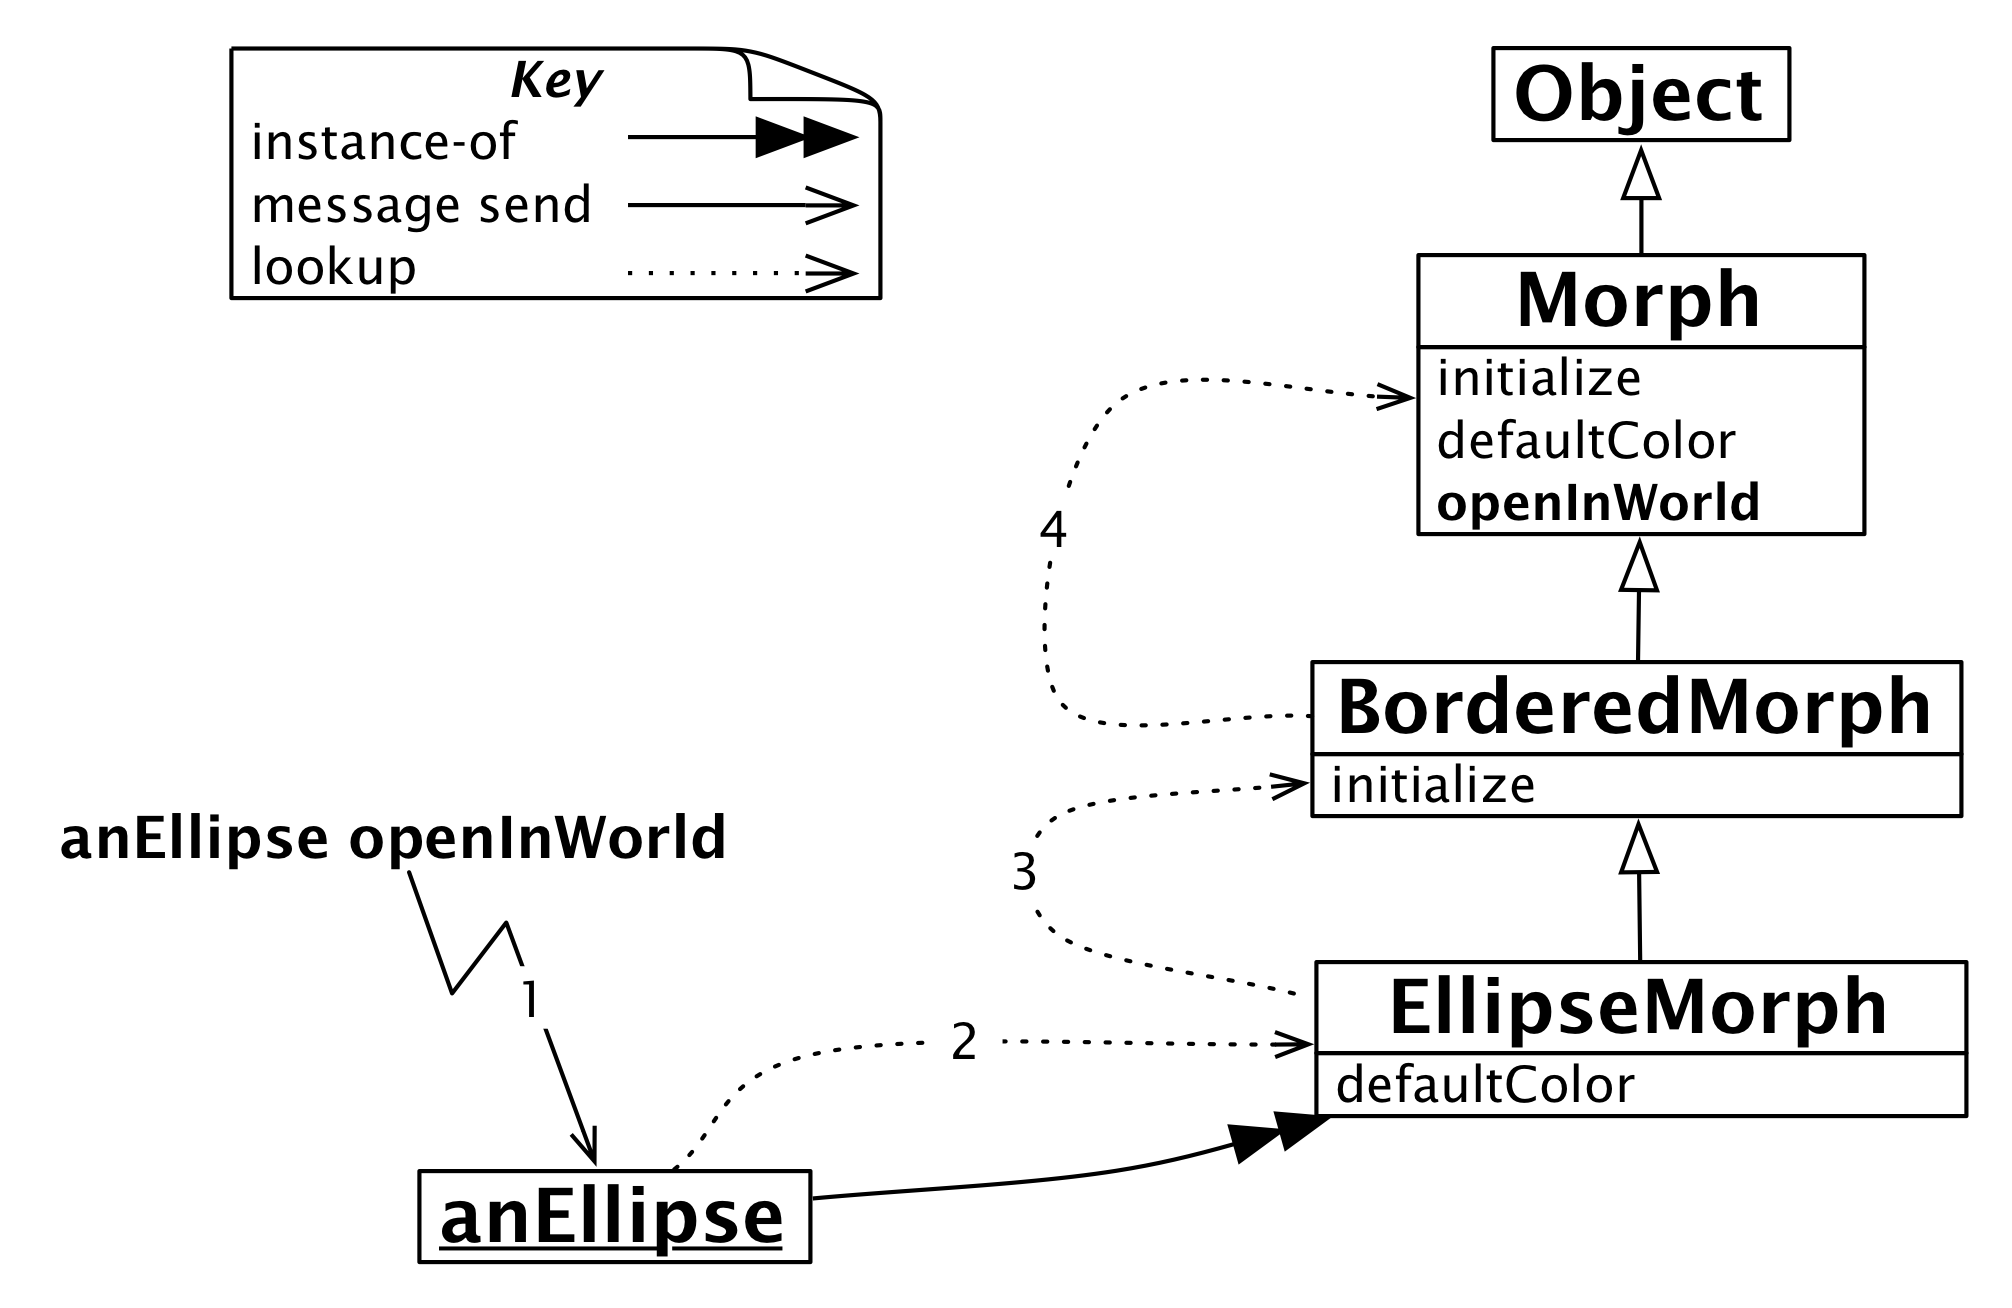
\includegraphics[width=0.8\textwidth]{/Users/sebastijan.kaplar/Desktop/PharoByExample/UpdatedPharoByExample/_result/pdf/PharoObjectModel/figures/openInWorldLookup.png}\caption{Method lookup follows the inheritance hierarchy\label{fig:openInWorldLookup}}\end{center}
\end{figure}

\section{Returning self}
Notice that \textcode{EllipseMorph\textgreater{}\textgreater{}defaultColor} explicitly returns \textcode{Color yellow},
whereas \textcode{Morph\textgreater{}\textgreater{}openInWorld} does not appear to return anything.

Actually a method \textit{always} answers a message with a value (which is, of
course, an object). The answer may be defined by the \textcode{\string^} construct in the
method, but if execution reaches the end of the method without executing a
\textcode{\string^}, the method still answers a value -- it answers the object that
received the message. We usually say that the method \textit{answers self}, because
in Pharo the pseudo-variable \textcode{self} represents the receiver of the message,
much like the keyword \textcode{this} in Java. Other languages, such as Ruby, by
default return the value of the last statement in the method. Again, this is not
the case in Pharo, instead you can imagine that a method without an explicit
return ends with \textcode{\string^ self}.

\begin{important}
\textcode{self} represents the receiver of the message.
\end{important}

This suggests that \textcode{openInWorld} is equivalent to \textcode{openInWorldReturnSelf},
defined below.

\begin{listing}[float, label=scr:openInWorldReturnSelf]{plain}{Explicitly returning \textcode{self}}
Morph >> openInWorld
    "Add this morph to the world."
    self openInWorld: self currentWorld
    ^ self
\end{listing}

Why is explicitly writing \textcode{\string^ self} not a so good thing to do? When you
return something explicitly, you are communicating that you are returning
something of interest to the sender. When you explicitly return \textcode{self}, you
are saying that you expect the sender to use the returned value. This is not the
case here, so it is best not to explicitly return \textcode{self}. We only return \textcode{self}
on special case to stress that the receiver is returned.

This is a common idiom in Pharo, which Kent Beck refers to as \textit{Interesting
return value}:

\textit{\symbol{34}Return a value only when you intend for the sender to use the value.\symbol{34}}

\begin{important}
By default (if not specified differently) a method returns the message receiver.
\end{important}
\section{Overriding and extension}
If we look again at the \textcode{EllipseMorph} class hierarchy in Figure
\ref{fig:openInWorldLookup}, we see that the classes \textcode{Morph} and \textcode{EllipseMorph}
both implement \textcode{defaultColor}. In fact, if we open a new morph (\textcode{Morph new
openInWorld}) we see that we get a blue morph, whereas an ellipse will be
yellow by default.

We say that \textcode{EllipseMorph} \textit{overrides} the \textcode{defaultColor} method that it
inherits from \textcode{Morph}. The inherited method no longer exists from the point of
view of \textcode{anEllipse}.

Sometimes we do not want to override inherited methods, but rather \textit{extend}
them with some new functionality, that is, we would like to be able to invoke
the overridden method \textit{in addition to} the new functionality we are defining
in the subclass. In Pharo, as in many object-oriented languages that support
single inheritance, this can be done with the help of \textcode{super} sends.

A frequent application of this mechanism is in the \textcode{initialize} method.
Whenever a new instance of a class is initialized, it is critical to also
initialize any inherited instance variables. However, the knowledge of how to do
this is already captured in the \textcode{initialize} methods of each of the superclass
in the inheritance chain. The subclass has no business even trying to initialize
inherited instance variables!

It is therefore good practice whenever implementing an \textcode{initialize} method to
send \textcode{super initialize} before performing any further initialization:

\begin{listing}[float, label=scr:morphinit]{plain}{Super initialize}
BorderedMorph >> initialize
    "initialize the state of the receiver"

    super initialize.
    self borderInitialize
\end{listing}

We need \textcode{super} sends to compose inherited behaviour that would otherwise be overridden.

\begin{important}
It is a good practice that an \textcode{initialize} method start by sending \textcode{super initialize}.
\end{important}
\section{Self sends and super sends}
\textcode{self} represents the receiver of the message and the lookup of the method
starts in the class of the receiver. Now what is \textcode{super}? \textcode{super} is
\textit{not} the superclass! It is a common and natural mistake to think this. It is
also a mistake to think that lookup starts in the superclass of the class of the
receiver.

\begin{important}
\textcode{self} represents the receiver of the message and the method lookup starts in the class of the receiver.
\end{important}
\subsection{How do \textcode{self} sends differ from \textcode{super} sends?}
Like \textcode{self}, \textcode{super} represents the receiver of the message. Yes you read it
well! The only thing that changes is the method lookup. Instead of lookup
starting in the class of the receiver, it starts in the \textit{superclass of the
class of the method where the \textcode{super} send occurs}.

\begin{important}
\textcode{super} represents the receiver of the message and the method lookup starts in the superclass of the class of the method where the \textcode{super} send occurs.
\end{important}

We shall see with the following example precisely how this works.
Imagine that we define the following three methods:

First we define the method \textcode{fullPrintOn:} on class \textcode{Morph} that just adds to
the stream the name of the class followed by the string ' new' - the idea is
that we could execute the resulting string and gets back an instance similar to
the receiver.

\begin{listing}[float, label=scr:morphfullPrintOn]{plain}{A \textcode{self} send}
Morph >> fullPrintOn: aStream
	aStream nextPutAll: self class name, ' new'
\end{listing}

Second we define the method \textcode{constructorString} that send the message \textcode{fullPrintOn:}.

\begin{listing}[float, label=scr:constructorString]{plain}{A \textcode{self} send}
Morph >> constructorString
    ^ String streamContents: [ :s | self fullPrintOn: s  ].
\end{listing}

Finally, we define the method \textcode{fullPrintOn:} on the class \textcode{BorderedMorph}
superclass of \textcode{EllipseMorph}. This new method extends the superclass behavior:
it invokes it and adds extra behavior.

\begin{listing}[float, label=scr:fullPrintOn]{plain}{Combining \textcode{super} and \textcode{self} sends}
BorderedMorph >> fullPrintOn: aStream
    aStream nextPutAll: '('.
    super fullPrintOn: aStream.
    aStream
        nextPutAll: ') setBorderWidth: ';
        print: borderWidth;
        nextPutAll: ' borderColor: ', (self colorString: borderColor)
\end{listing}

Consider the message \textcode{constructorString} sent to an instance of \textcode{EllipseMorph}:

\begin{displaycode}{plain}
EllipseMorph new constructorString
>>> '(EllipseMorph new) setBorderWidth: 1 borderColor: Color black'
\end{displaycode}

How exactly is this result obtained through a combination of \textcode{self} and
\textcode{super} sends? First, \textcode{anEllipse constructorString} will cause the method
\textcode{constructorString} to be found in the class \textcode{Morph}, as shown in Figure
\ref{fig:constructorStringLookup}.


\begin{figure}

\begin{center}
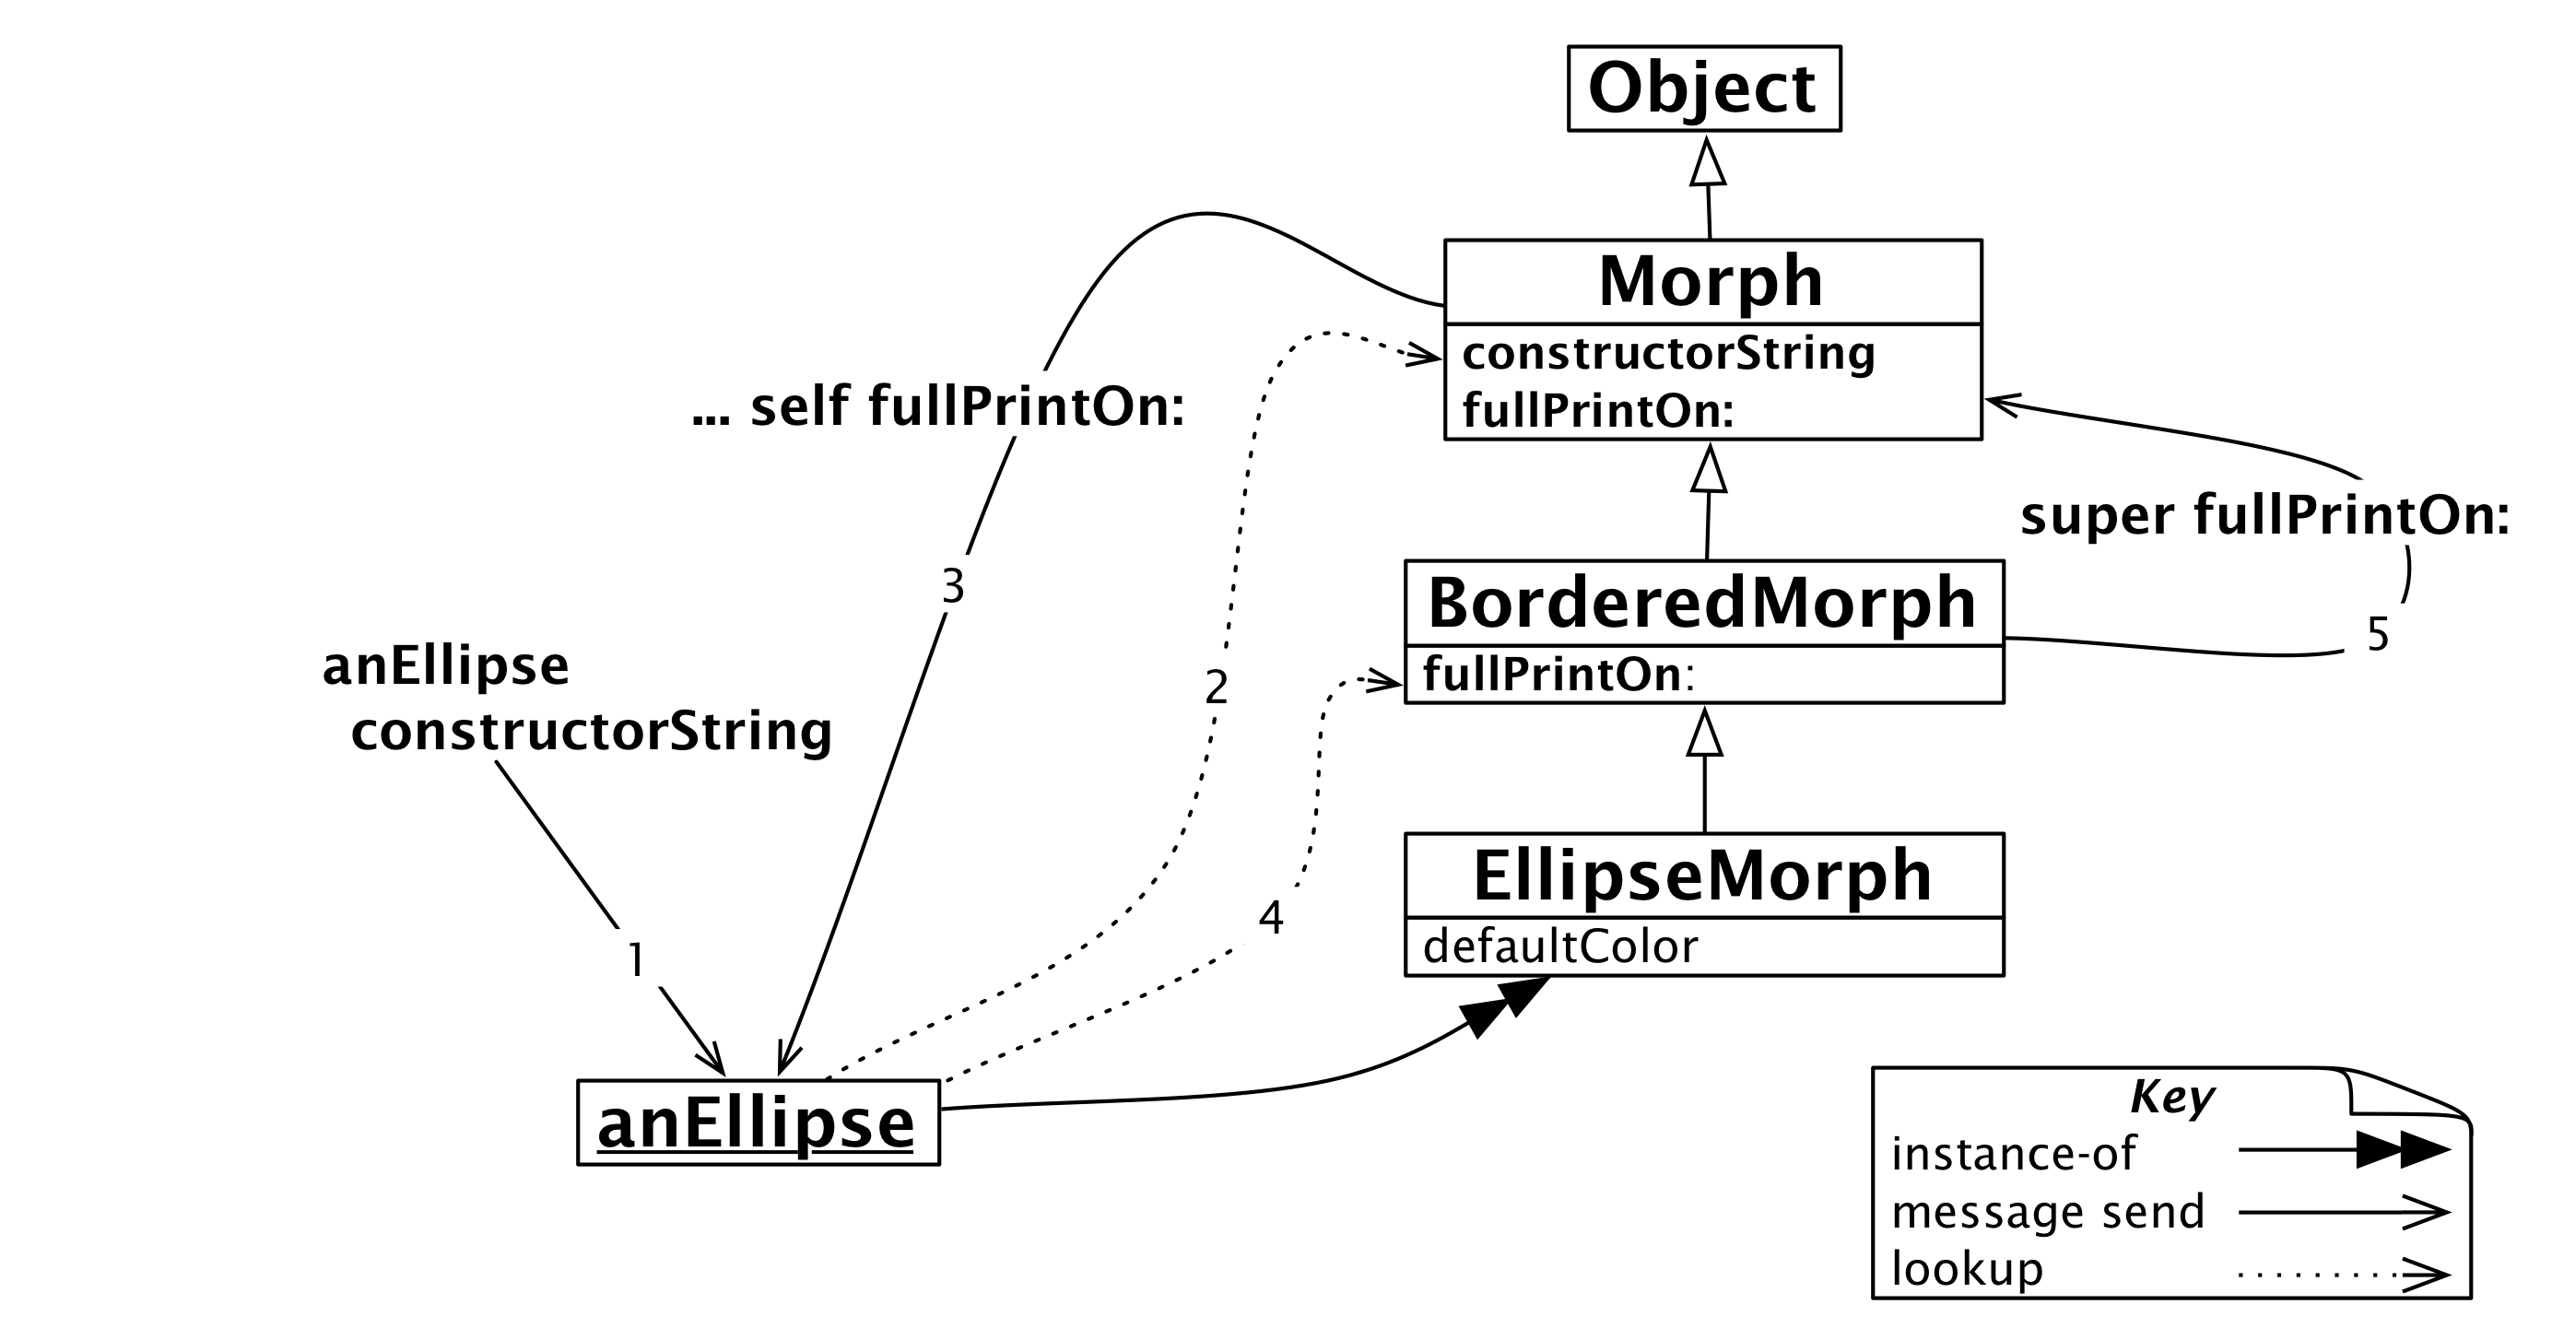
\includegraphics[width=0.9\textwidth]{/Users/sebastijan.kaplar/Desktop/PharoByExample/UpdatedPharoByExample/_result/pdf/PharoObjectModel/figures/constructorStringLookup.png}\caption{\textcode{self} and \textcode{super} sends\label{fig:constructorStringLookup}}\end{center}
\end{figure}


The method \textcode{Morph\textgreater{}\textgreater{}constructorString} performs a \textcode{self} send of
\textcode{fullPrintOn:}. The message \textcode{fullPrintOn:} is looked up starting in the
class \textcode{EllipseMorph}, and the method \textcode{BorderedMorph\textgreater{}\textgreater{}fullPrintOn:} is found
in \textcode{BorderedMorph} (see Figure \ref{fig:constructorStringLookup}). What is
critical to notice is that the \textcode{self} send causes the method lookup to start
again in the class of the receiver, namely the class of \textcode{anEllipse}.

At this point, \textcode{BorderedMorph\textgreater{}\textgreater{}fullPrintOn:} does a \textcode{super} send to extend
the \textcode{fullPrintOn:} behaviour it inherits from its superclass. Because this is
a \textcode{super} send, the lookup now starts in the superclass of the class where the
\textcode{super} send occurs, namely in \textcode{Morph}. We then immediately find and
evaluate \textcode{Morph\textgreater{}\textgreater{}fullPrintOn:}.
\subsection{Stepping back}
A \textcode{self} send is dynamic in the sense that by looking at the method containing
it, we cannot predict which method will be executed. Indeed an instance of a
subclass may receive the message containing the self expression and redefine the
method in that subclass. Here \textcode{EllipseMorph} could redefine the method
\textcode{fullPrintOn:} and this method would be executed by method
\textcode{constructorString}. Note that by only looking at the method
\textcode{constructorString}, we cannot predict which \textcode{fullPrintOn:} method (either
the one of \textcode{EllipseMorph}, \textcode{BorderedMorph}, or \textcode{Morph}) will be executed
when executing the method \textcode{constructorString}, since it depends on the
receiver the \textcode{constructorString} message.

\begin{important}
A \textcode{self} send triggers a \textit{method lookup starting in the class of the receiver.} A \textcode{self} send is dynamic in the sense that by looking at the method containing it, we cannot predict which method will be executed.
\end{important}

Note that the \textcode{super} lookup did not start in the superclass of the receiver.
This would have caused lookup to start from \textcode{BorderedMorph}, resulting in an
infinite loop!

If you think carefully about \textcode{super} send and Figure
\ref{fig:constructorStringLookup}, you will realize that \textcode{super} bindings are
static: all that matters is the class in which the text of the \textcode{super} send is
found. By contrast, the meaning of \textcode{self} is dynamic: it always represents the
receiver of the currently executing message. This means that \textit{all} messages
sent to \textcode{self} are looked up by starting in the receiver's class.

\begin{important}
A \textcode{super} send triggers a method lookup starting in the \textit{superclass of the class of the method performing the \textcode{super} send}. We say that super sends are \textit{static} because just looking at the method we know the class where the lookup should start (the class above the class containing the method).
\end{important}
\section{Message not understood}
What happens if the method we are looking for is not found?

Suppose we send the message \textcode{foo} to our ellipse. First the normal method
lookup would go through the inheritance chain all the way up to \textcode{Object} (or
rather \textcode{ProtoObject}) looking for this method. When this method is not found,
the virtual machine will cause the object to send \textcode{self doesNotUnderstand:
\#foo}. (See Figure \ref{fig:fooNotFound}.)


\begin{figure}

\begin{center}
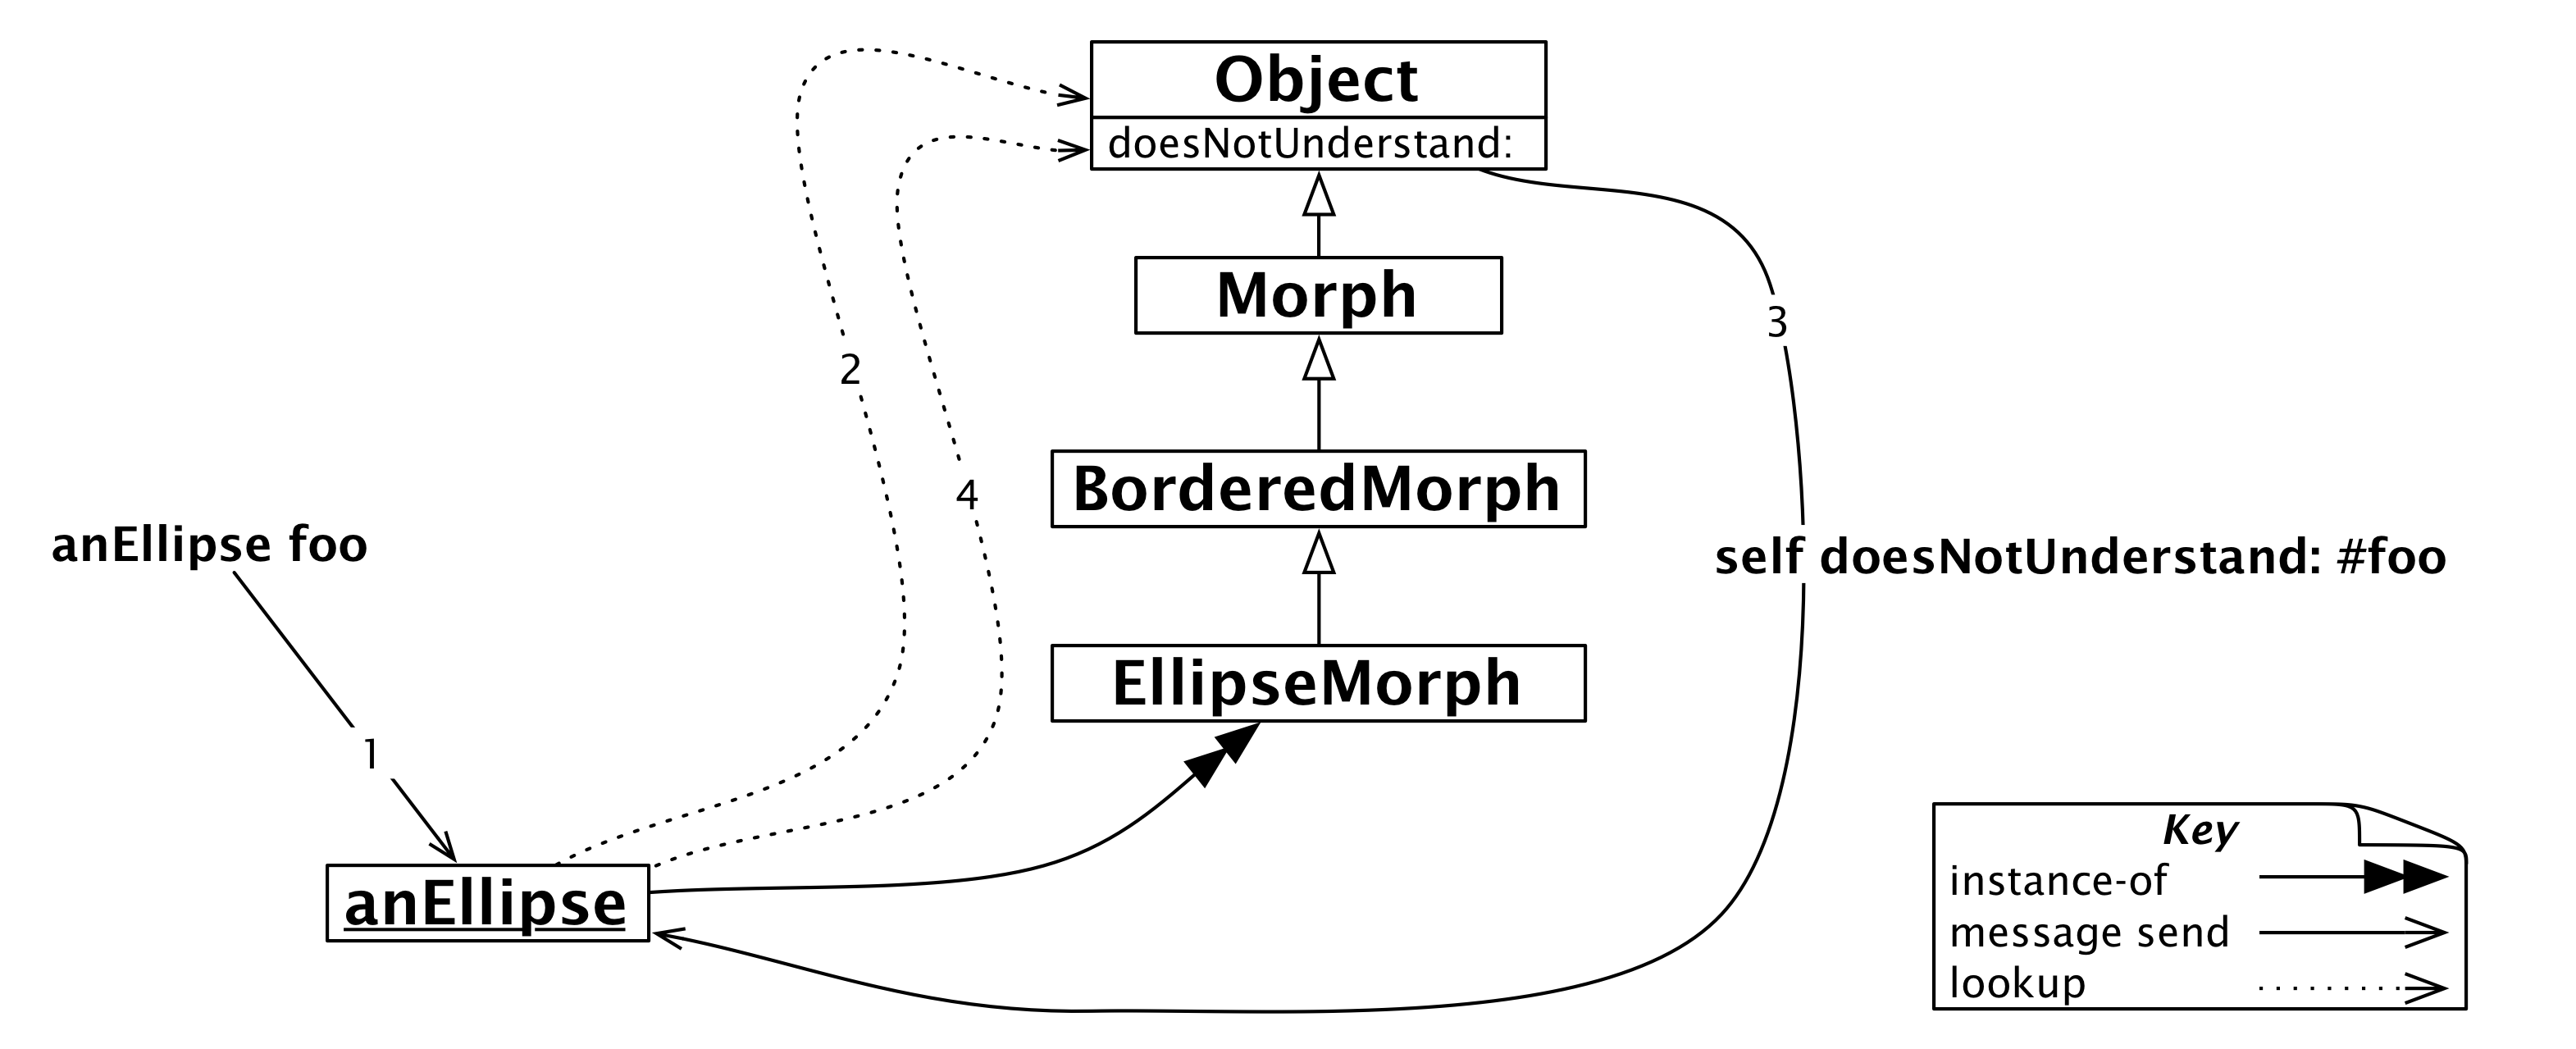
\includegraphics[width=0.8\textwidth]{/Users/sebastijan.kaplar/Desktop/PharoByExample/UpdatedPharoByExample/_result/pdf/PharoObjectModel/figures/fooNotFound.png}\caption{Message \textcode{foo} is not understood\label{fig:fooNotFound}}\end{center}
\end{figure}


Now, this is a perfectly ordinary, dynamic message send, so the lookup starts
again from the class \textcode{EllipseMorph}, but this time searching for the method
\textcode{doesNotUnderstand:}. As it turns out, \textcode{Object} implements
\textcode{doesNotUnderstand:}. This method will create a new \textcode{MessageNotUnderstood}
object which is capable of starting a Debugger in the current execution context.

Why do we take this convoluted path to handle such an obvious error? Well, this
offers developers an easy way to intercept such errors and take alternative
action. One could easily override the method \textcode{Object\textgreater{}\textgreater{}doesNotUnderstand:} in
any subclass of \textcode{Object} and provide a different way of handling the error.

In fact, this can be an easy way to implement automatic delegation of messages
from one object to another. A \textcode{Delegator} object could simply delegate all
messages it does not understand to another object whose responsibility it is to
handle them, or raise an error itself!
\chapter{Shared variables}
Now we will look at an aspect of Pharo that is not so easily covered by our five
rules: shared variables.

Pharo provides three kinds of shared variables:

\textbf{1.} \textit{Globally} shared variables.

\textbf{2.} \textit{Class variables}: variables shared between instances and classes. (Not
to be confused with class instance variables, discussed earlier).

\textbf{3.} \textit{Pool variables}: variables shared amongst a group of classes,

The names of all of these shared variables start with a capital letter, to warn
us that they are indeed shared between multiple objects.
\section{Global variables}
In Pharo, all global variables are stored in a namespace called \textcode{Smalltalk},
which is implemented as an instance of the class \textcode{SystemDictionary}. Global
variables are accessible everywhere. Every class is named by a global variable.
In addition, a few globals are used to name special or commonly useful objects.

The variable \textcode{Processor} names an instance of \textcode{ProcessScheduler}, the main
process schedler of Pharo.

\begin{displaycode}{plain}
Processor class
>>> ProcessorScheduler
\end{displaycode}
\subsection{Other useful global variables}
\textbf{\textcode{Smalltalk}} is the instance of \textcode{SmalltalkImage}. It contains many
functionality to manage the system. In particular it holds a reference to the
main namespace \textcode{Smalltalk globals}. This namespace includes \textcode{Smalltalk}
itself since it is a global variable. The keys to this namespace are the
symbols that name the global objects in Pharo code. So, for example:

\begin{displaycode}{plain}
Smalltalk globals at: #Boolean
>>> Boolean
\end{displaycode}

Since \textcode{Smalltalk} is itself a global variable:

\begin{displaycode}{plain}
Smalltalk globals at: #Smalltalk
>>> Smalltalk
\end{displaycode}

\begin{displaycode}{plain}
(Smalltalk globals at: #Smalltalk) == Smalltalk
>>> true
\end{displaycode}

\textbf{\textcode{World}} is an instance of \textcode{PasteUpMorph} that represents the screen.
\textcode{World bounds} answers a rectangle that defines the whole screen space; all
Morphs on the screen are submorphs of \textcode{World}.

\textbf{\textcode{ActiveHand}} is the current instance of \textcode{HandMorph}, the graphical
representation of the cursor. \textcode{ActiveHand}'s submorphs hold anything being
dragged by the mouse.

\textbf{\textcode{Undeclared}} is another dictionary, which contains all the undeclared
variables. If you write a method that references an undeclared variable, the
browser will normally prompt you to declare it, for example as a global or as an
instance variable of the class. However, if you later delete the declaration,
the code will then reference an undeclared variable. Inspecting \textcode{Undeclared}
can sometimes help explain strange behaviour!
\subsection{Using globals in your code}
The recommended practice is to strictly limit the use of global variables. It is
usually better to use class instance variables or class variables, and to
provide class methods to access them. Indeed, if Pharo were to be implemented
from scratch today, most of the global variables that are not classes would be
replaced by singletons.

The usual way to define a global is just to perform \textcode{Do it} on an assignment
to a capitalized but undeclared identifier. The parser will then offer to
declare the global for you. If you want to define a global programmatically,
just execute \textcode{Smalltalk globals at: \#AGlobalName put: nil}. To remove it,
execute \textcode{Smalltalk globals removeKey: \#AGlobalName}.
\section{Class variables}\label{sec:classVars}
Sometimes we need to share some data amongst all the instances of a class and
the class itself. This is possible using \textit{class variables}. The term \textit{class
variable} indicates that the lifetime of the variable is the same as that of
the class. However, what the term does not convey is that these variables are
shared amongst all the instances of a class as well as the class itself, as
shown in Figure \ref{fig:privateSharedVar}. Indeed, a better name would have been
\textit{shared variables} since this expresses more clearly their role, and also
warns of the danger of using them, particularly if they are modified.


\begin{figure}

\begin{center}
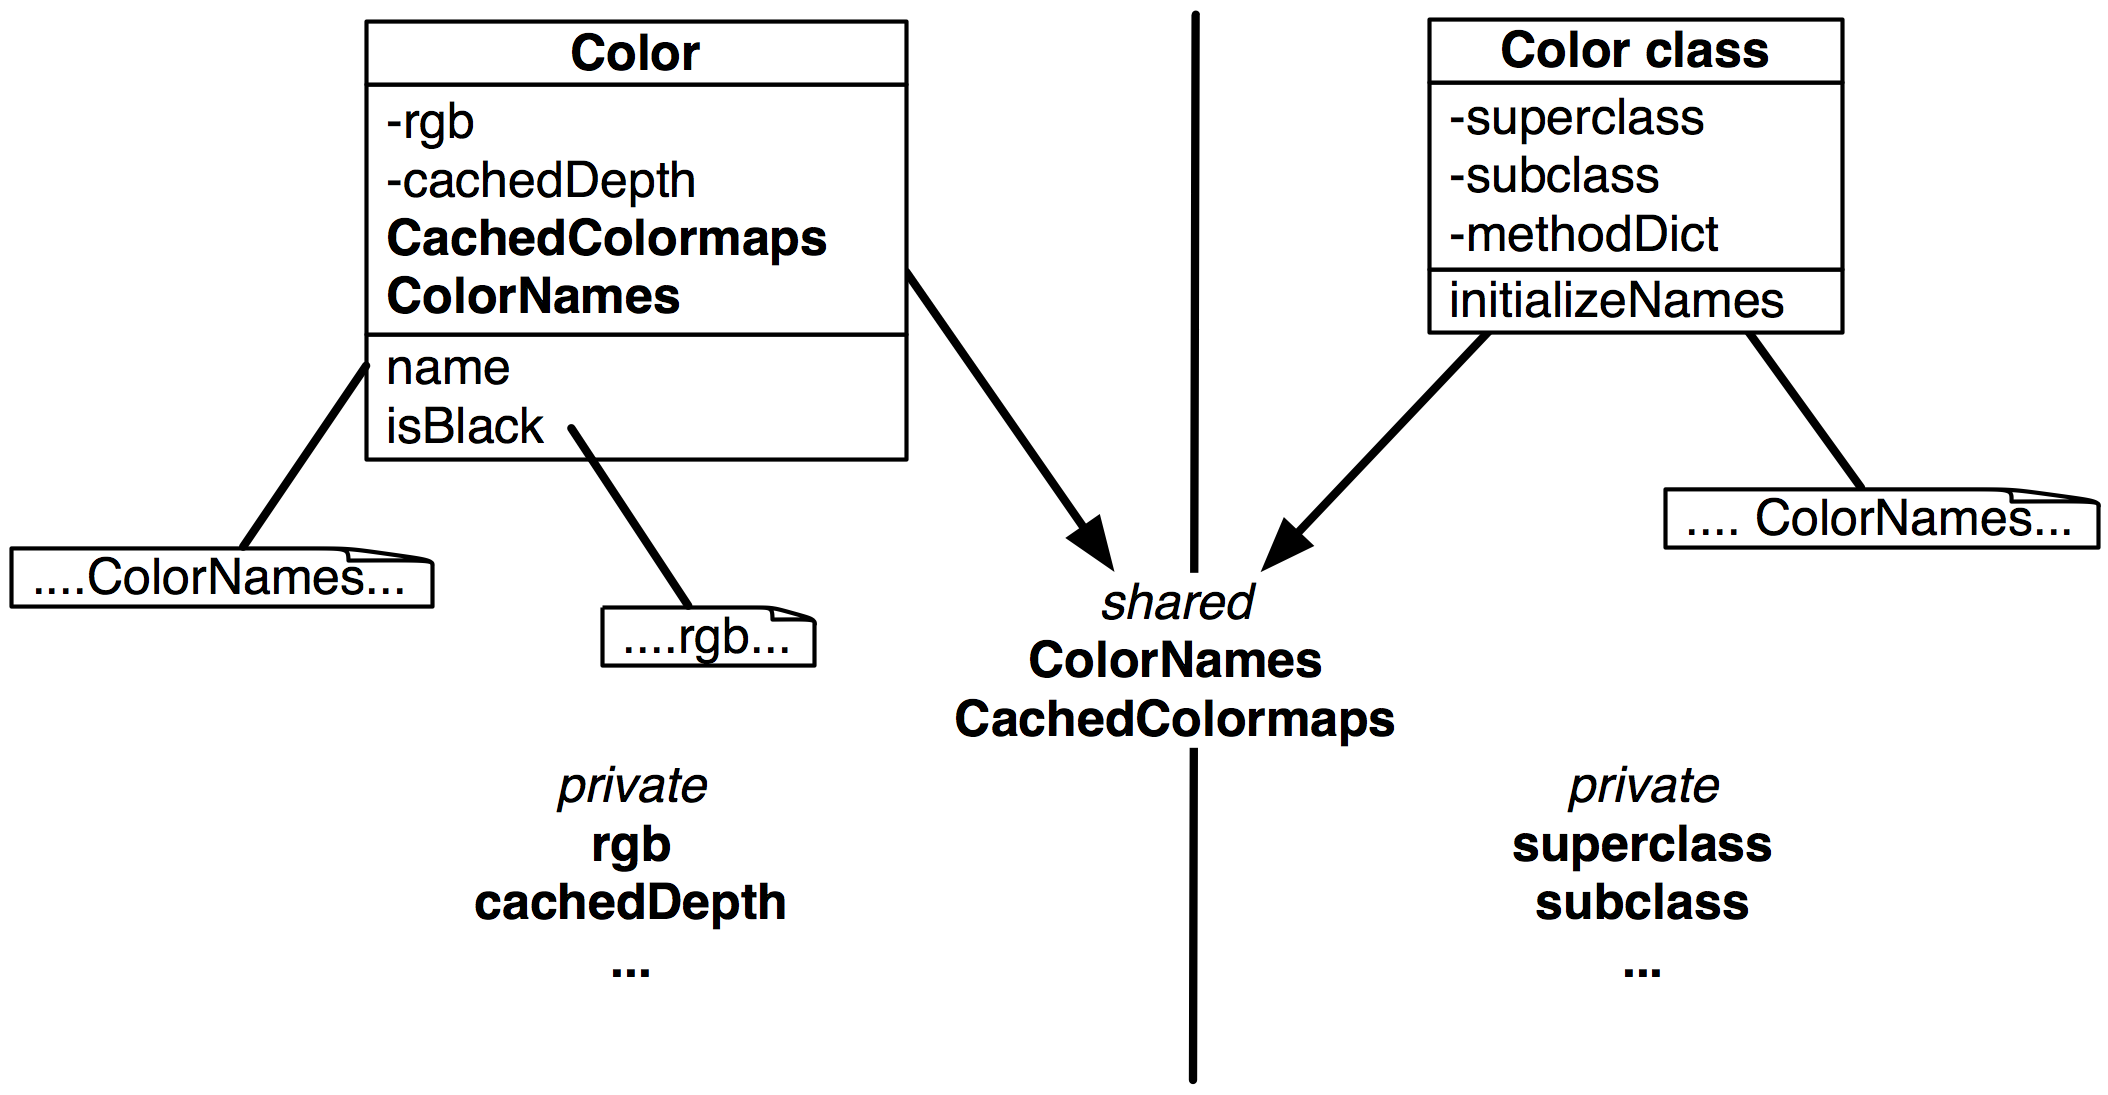
\includegraphics[width=0.7\textwidth]{/Users/sebastijan.kaplar/Desktop/PharoByExample/UpdatedPharoByExample/_result/pdf/PharoObjectModel/figures/privateSharedVarColor.png}\caption{Instance and class methods accessing different variables\label{fig:privateSharedVar}}\end{center}
\end{figure}


In Figure \ref{fig:privateSharedVar} we see that \textcode{rgb} and \textcode{cachedDepth} are
instance variables of \textcode{Color}, hence only accessible to instances of
\textcode{Color}. We also see that \textcode{superclass}, \textcode{subclass}, \textcode{methodDict} and so
on are \textit{class instance variables}, i.e., instance variables only accessible to
the \textcode{Color} class.

But we can also see something new: \textcode{ColorRegistry} and \textcode{CachedColormaps} are
\textit{class variables} defined for \textcode{Color}. The capitalization of these variables
gives us a hint that they are shared. In fact, not only may all instances of
\textcode{Color} access these shared variables, but also the \textcode{Color} class itself,
\textit{and any of its subclasses}. Both instance methods and class methods can
access these shared variables.

A class variable is declared in the class definition template. For example, the
class \textcode{Color} defines a large number of class variables to speed up color
creation; its definition is shown below.

\begin{listing}[float, label=scr:classDefColor]{plain}{Color and its class variables}
Object subclass: #Color
	instanceVariableNames: 'rgb cachedDepth cachedBitPattern alpha'
	classVariableNames: 'BlueShift CachedColormaps ColorRegistry ComponentMask GrayToIndexMap GreenShift HalfComponentMask IndexedColors
    MaskingMap RandomStream RedShift'
	package: 'Graphics-Primitives'
\end{listing}

The class variable \textcode{ColorRegistry} is an instance of \textcode{IdentityDictionary}
containing the frequently-used colors, referenced by name. This dictionary is
shared by all the instances of \textcode{Color}, as well as the class itself. It is
accessible from all the instance and class methods.
\subsection{Class initialization}
The presence of class variables raises the question: how do we initialize them?

One solution is lazy initialization (discussed earlier in this chapter). This
can be done by introducing an accessor method which, when executed, initializes
the variable if it has not yet been initialized. This implies that we must use
the accessor all the time and never use the class variable directly. This
furthermore imposes the cost of the accessor send and the initialization test.
It also arguably defeats the point of using a class variable, since in fact it
is no longer shared.

Another solution is to override the class method \textcode{initialize} (we've seen this
before in the Dog example).

\begin{listing}[float, label=scr:colorClassInit]{plain}{Initializing the \textcode{Color} class}
Color class >> initialize
    ...
    self initializeColorRegistry.
    ...
\end{listing}

If you adopt this solution, you will need to remember to invoke the
\textcode{initialize} method after you define it (by evaluating \textcode{Color initialize}).
Although class side \textcode{initialize} methods are executed automatically when code
is loaded into memory (from a Monticello repository, for example), they are
\textit{not} executed automatically when they are first typed into the browser and
compiled, or when they are edited and re-compiled.
\section{Pool variables}
Pool variables are variables that are shared between several classes that may
not be related by inheritance. Pool variables were originally stored in pool
dictionaries; now they should be defined as class variables of dedicated classes
(subclasses of \textcode{SharedPool}). Our advice is to avoid them; you will need them
only in rare and specific circumstances. Our goal here is therefore to explain
pool variables just enough so that you can understand them when you are reading
code.

A class that accesses a pool variable must mention the pool in its class
definition. For example, the class \textcode{Text} indicates that it is using the pool
dictionary \textcode{TextConstants}, which contains all the text constants such as
\textcode{CR} and \textcode{LF}. This dictionary has a key \textcode{\#CR} that is bound to the value
\textcode{Character cr}, i.e., the carriage return character.

\begin{listing}[float, label=scr:textPoolDict]{plain}{Pool dictionaries in the \textcode{Text} class}
ArrayedCollection subclass: #Text
        instanceVariableNames: 'string runs'
        classVariableNames: ''
        poolDictionaries: 'TextConstants'
        package: 'Collections-Text'
\end{listing}

This allows methods of the class \textcode{Text} to access the \textit{keys} of the
dictionary in the method body \textit{directly}, i.e., by using variable syntax
rather than an explicit dictionary lookup. For example, we can write the
following method.

\begin{listing}[float, label=scr:textTestCR]{plain}{\textcode{Text\textgreater{}\textgreater{}testCR}}
Text >> testCR
    ^ CR == Character cr
\end{listing}

Once again, we recommend that you avoid the use of pool variables and pool
dictionaries.
\chapter{Internal object implementation note}
Here is an implementation note for people that really want to go deep inside the
way Pharo represents internally objects. The implementation distinguished
between two different kinds of objects: \# Objects with zero or more fields that
are passed by reference and exist on the Pharo heap. \# Immediate objects that
are passed by value. Depending on version, these are a range of the integers
called SmallInteger, all \textcode{Character} objects and possibly a sub-range of
64-bit floating-point numbers called \textcode{SmallFloat64}. In the implementation,
such immediate objects occupy an object pointer, most of whose bits encode the
immediate's value and some of the bits encode the object's class.

The first kind of object, an ordinary object, comes in a number of varieties:

\begin{enumerate}
\item Normal objects that have zero or more named instance variables, such as \textcode{Point} which has an x and a y instance variable. Each instance variable holds an object pointer, which can be a reference to another ordinary object or an immediate.
\item Indexable objects like arrays that have zero or more indexed instance variables numbered from 1 to N. Each indexed instance variable holds an object pointer, which can be a reference to another ordinary object or an immediate.  Indexable objects are accessed using the messages \textcode{at:} and \textcode{at:put:}. For example \textcode{((Array new: 1) at: 1 put: 2; at: 1)} answers 2.
\item Objects like Closure or Context that have both named instance variables and indexed instance variables. In the object, the indexed instance variables follow the named instance variables.
\item Objects like \textcode{ByteString} or \textcode{Bitmap} that have indexed instance variables numbered from 1 to N that contain raw data. Each datum may occupy 8, 16 or 32-bits, depending on its class definition. The data can be accessed as either integers, characters or floating-point numbers, depending on how methods \textcode{at:} and \textcode{at:put:} are implemented. The \textcode{at:} and \textcode{at:put:} methods convert between Pharo objects and raw data, hiding the internal representation, but allowing the system to represent efficiently data such as strings, and bitmaps.
\end{enumerate}

The beauty of Pharo is that you normally don't need to care about the
differences between these three kinds of object.
\chapter{Chapter summary}
The object model of Pharo is both simple and uniform.
Everything is an object, and pretty much everything happens by sending messages.

\begin{itemize}
\item Everything is an object. Primitive entities like integers are objects, but also classes are first-class objects.
\item Every object is an instance of a class. Classes define the structure of their instances via \textit{private} instance variables and the behaviour of their instances via \textit{public} methods. Each class is the unique instance of its metaclass. Class variables are private variables shared by the class and all the instances of the class. Classes cannot directly access instance variables of their instances, and instances cannot access instance variables of their class. Accessors must be defined if this is needed.
\item Every class has a superclass. The root of the single inheritance hierarchy is \textcode{ProtoObject}. Classes you define, however, should normally inherit from \textcode{Object} or its subclasses. There is no syntax for defining abstract classes. An abstract class is simply a class with an abstract method (one whose implementation consists of the expression \textcode{self subclassResponsibility}). Although Pharo supports only single inheritance, it is easy to share implementations of methods by packaging them as \textit{traits}.
\item Everything happens by sending messages. We do not \textit{call methods}, we \textit{send messages}. The receiver then chooses its own method for responding to the message.
\item Method lookup follows the inheritance chain; \textcode{self} sends are dynamic and start the method lookup in the class of the receiver, whereas \textcode{super} sends start the method lookup in the superclass of class in which the \textcode{super} send is written. From this perspective \textcode{super} sends are more static than \textcode{self} sends.
\item There are three kinds of shared variables. Global variables are accessible everywhere in the system. Class variables are shared between a class, its subclasses and its instances. Pool variables are shared between a selected set of classes. You should avoid shared variables as much as possible.
\end{itemize}


% lulu requires an empty page at the end. That's why I'm using
% \backmatter here.
\backmatter

% Index would go here

\end{document}
